\section{Experiments}

We evaluated our method on several image-video pairs. For a baseline comparison, we used the same inputs on our off-the-shelf model to provide a fair comparison (\cref{fig:results}).

\begin{table*}[t]\centering
    \begin{tabular}{c|c|c|c}
        Input Image                                                 & Driving Video                                               & Baseline (VideoComposer)                                    & Ours                                                          \\ \midrule
        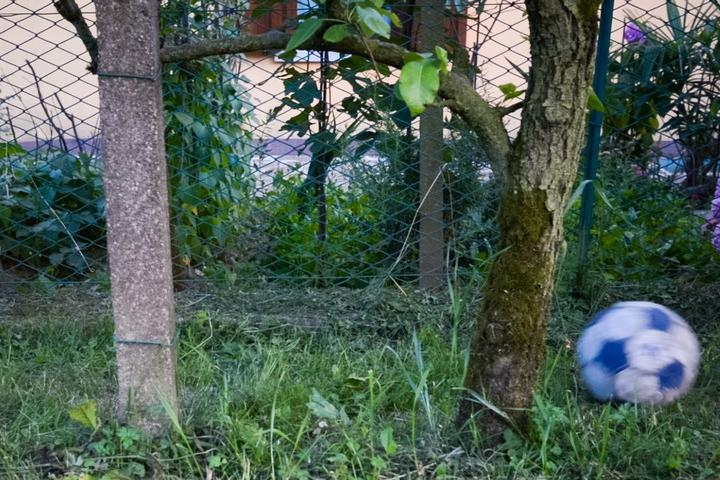
\includegraphics[width=0.23\linewidth]{media/ball/ii.jpg}   & 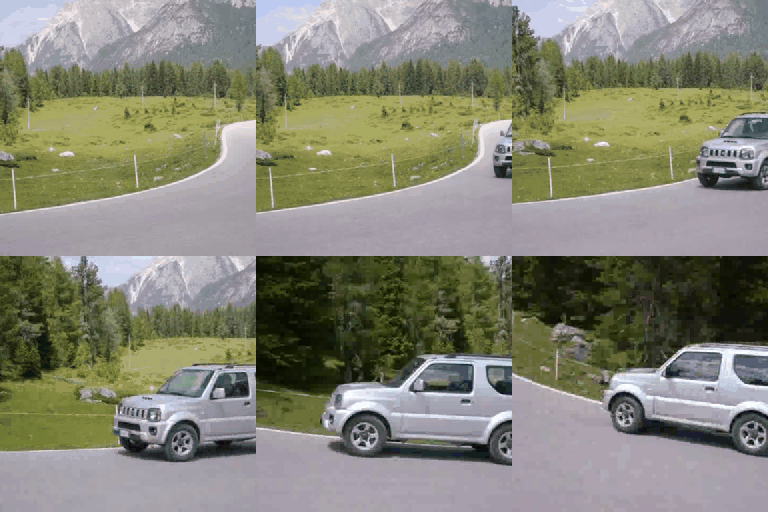
\includegraphics[width=0.23\linewidth]{media/ball/dv.png}   & 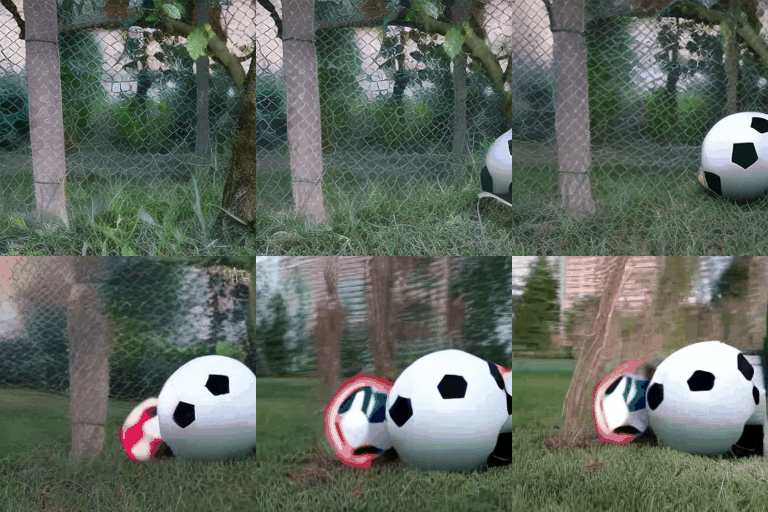
\includegraphics[width=0.23\linewidth]{media/ball/vc.png}   & 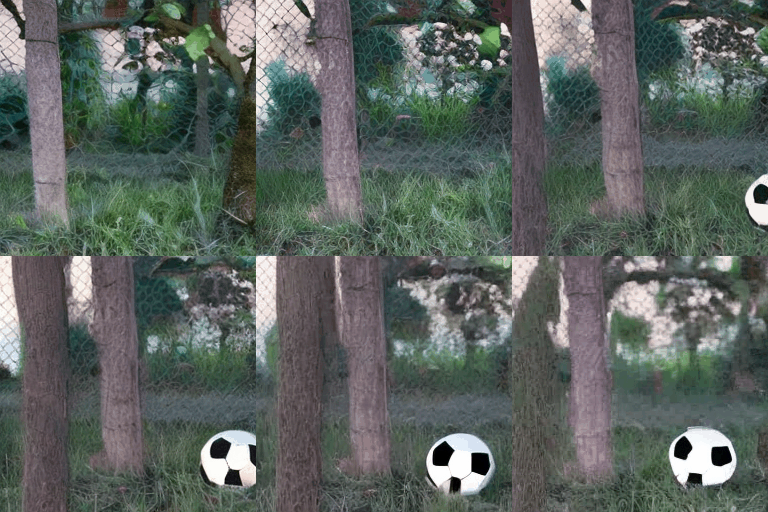
\includegraphics[width=0.23\linewidth]{media/ball/ours.png}   \\
        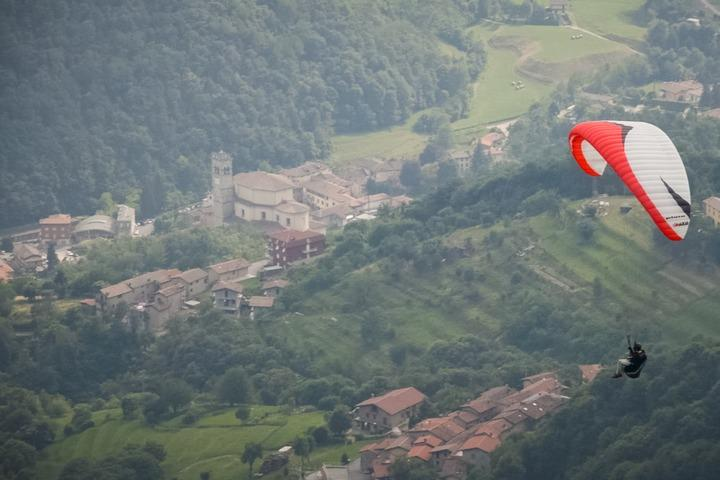
\includegraphics[width=0.23\linewidth]{media/glider/ii.jpg} & 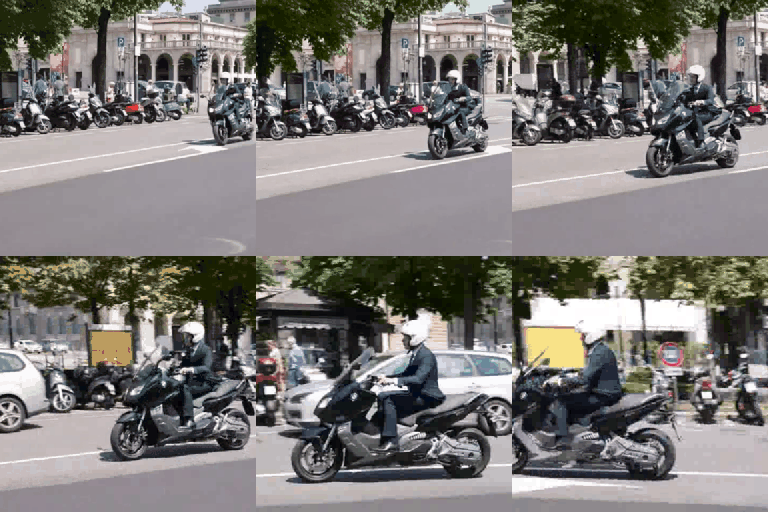
\includegraphics[width=0.23\linewidth]{media/glider/dv.png} & 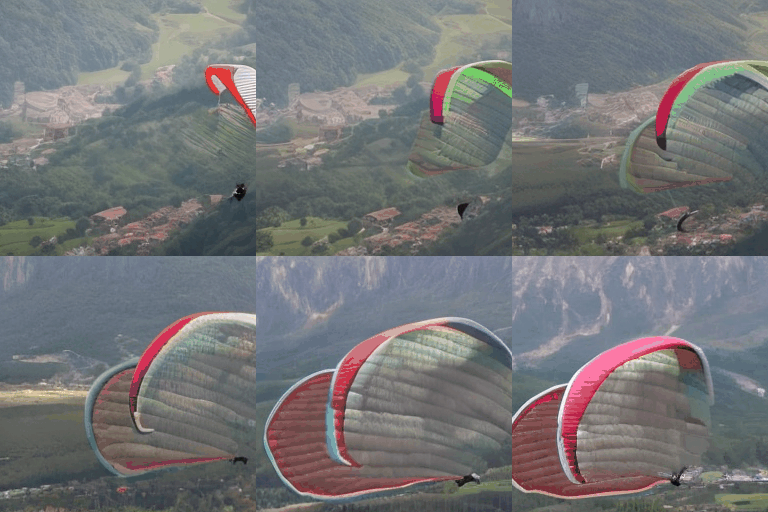
\includegraphics[width=0.23\linewidth]{media/glider/vc.png} & 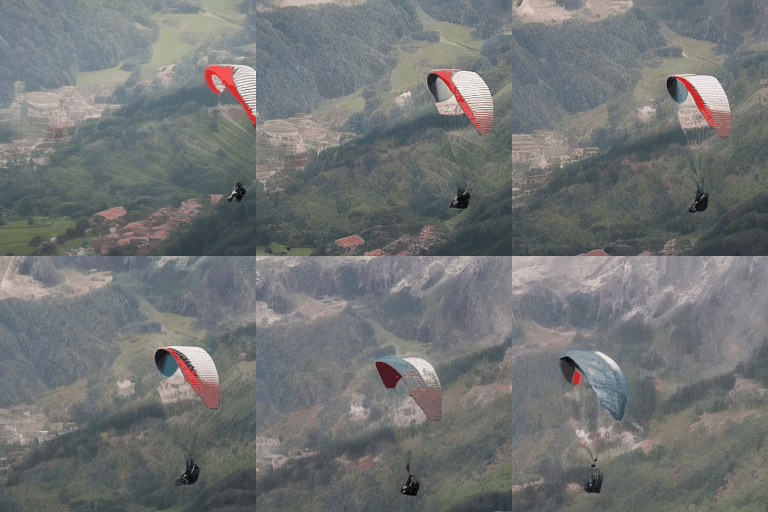
\includegraphics[width=0.23\linewidth]{media/glider/ours.png} \\
        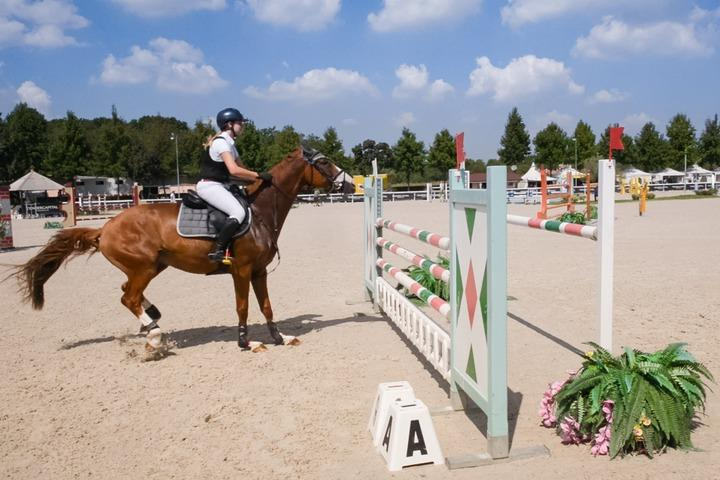
\includegraphics[width=0.23\linewidth]{media/horse/ii.jpg}  & 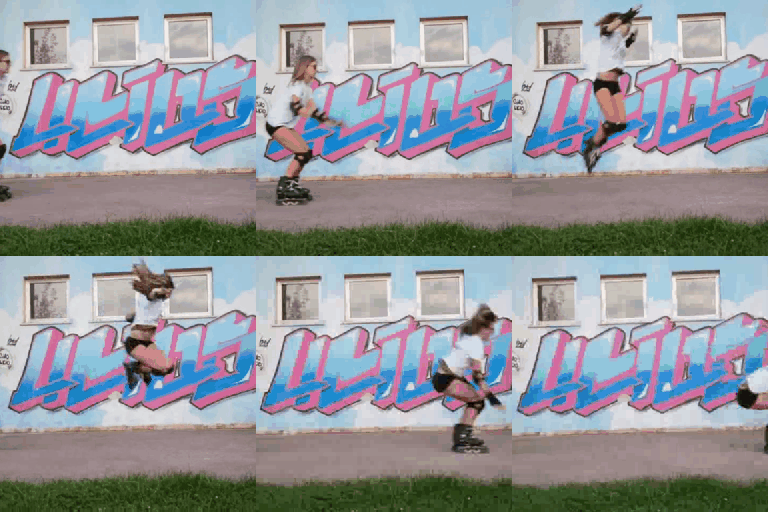
\includegraphics[width=0.23\linewidth]{media/horse/dv.png}  & 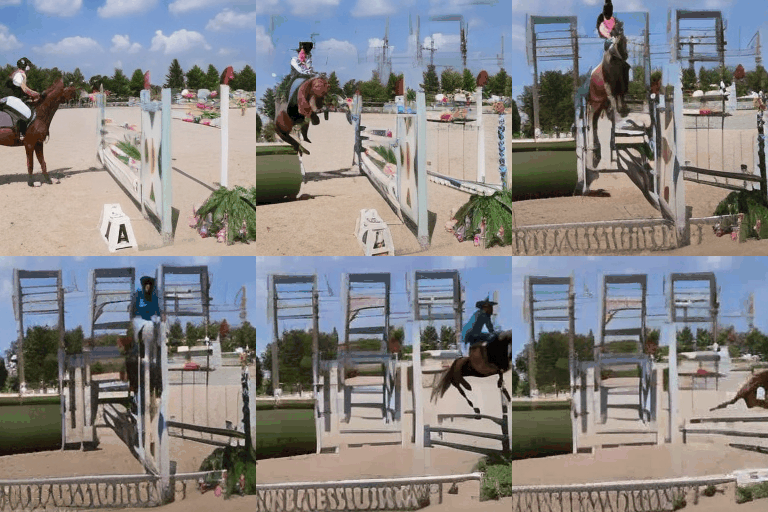
\includegraphics[width=0.23\linewidth]{media/horse/vc.png}  & 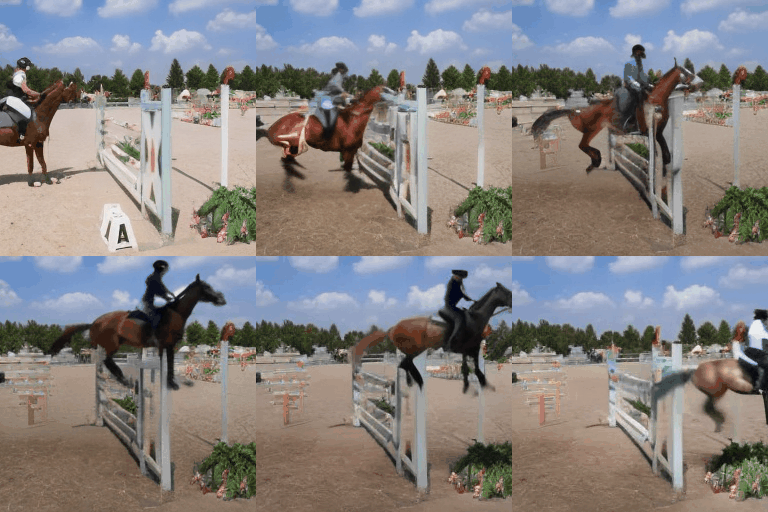
\includegraphics[width=0.23\linewidth]{media/horse/ours.png}  \\
        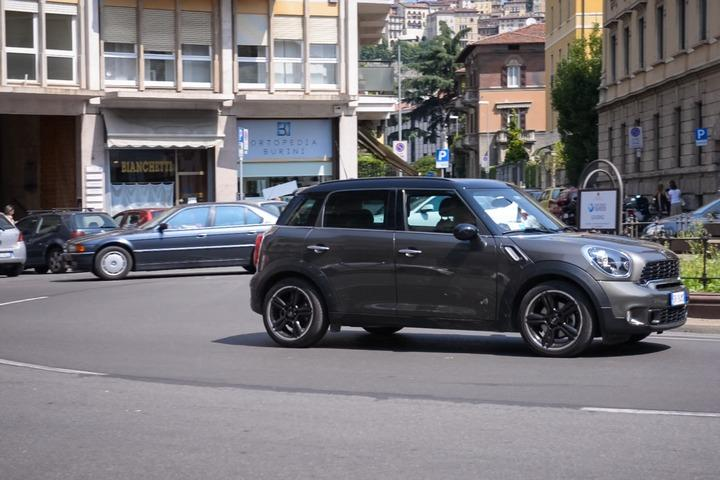
\includegraphics[width=0.23\linewidth]{media/car/ii.jpg}    & 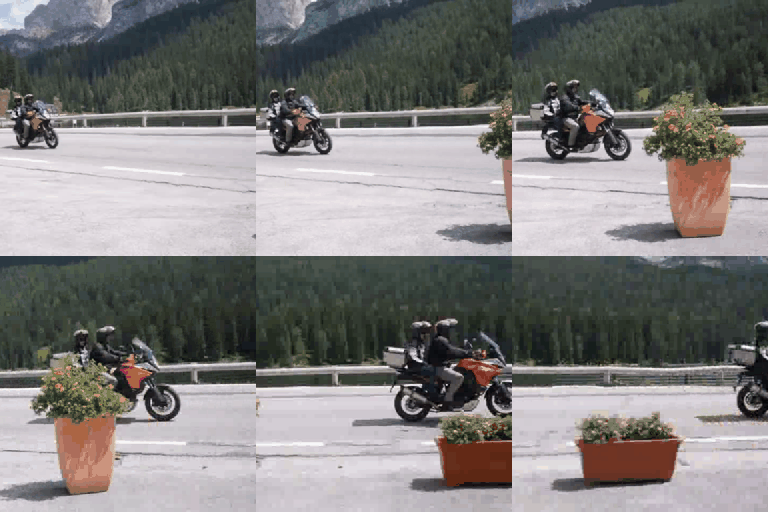
\includegraphics[width=0.23\linewidth]{media/car/dv.png}    & 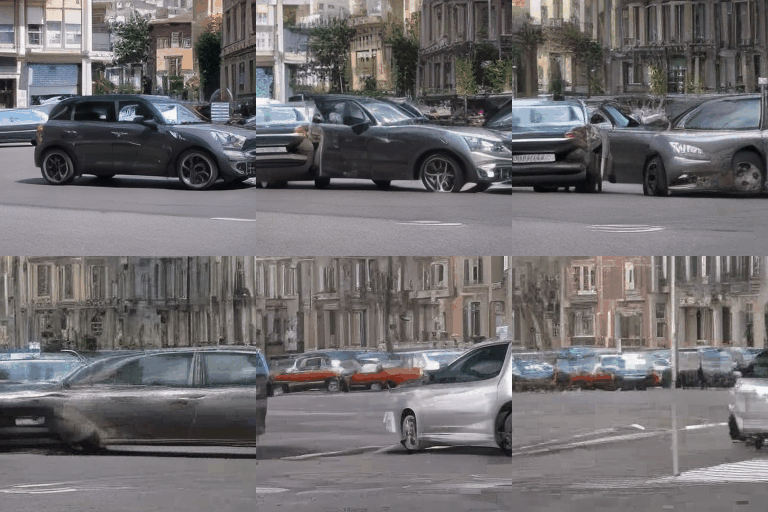
\includegraphics[width=0.23\linewidth]{media/car/vc.png}    & 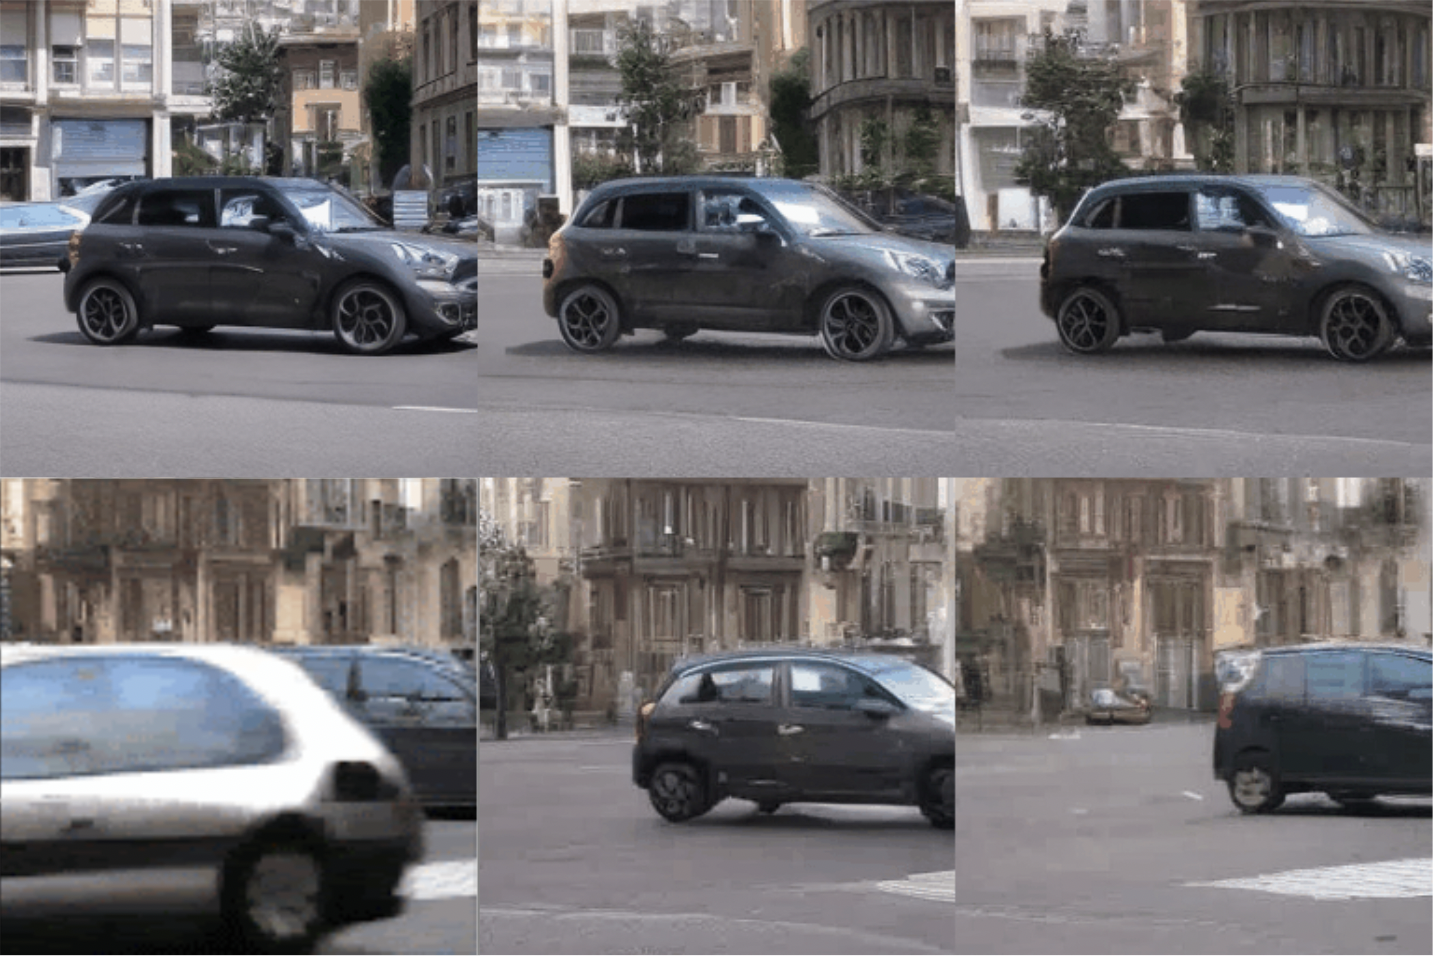
\includegraphics[width=0.23\linewidth]{media/car/ours.png}    \\
    \end{tabular}
    \caption{A side-by-side comparison of results from our method and the baseline.}
    \label{fig:results}
\end{table*}
